\documentclass[autodetect-engine,dvipdfmx-if-dvi,ja=standard, 12pt]{bxjsarticle}

% 二段組にするとき
% \documentclass[twocolumn,autodetect-engine,dvipdfmx-if-dvi,ja=standard]{bxjsarticle}

\usepackage{graphicx}        %図を表示するのに必要
\usepackage{color}           %jpgなどを表示するのに必要
\usepackage{amsmath,amssymb} %数学記号を出すのに必要
\usepackage{setspace}
\usepackage{cases}
\usepackage{here}
\usepackage{fancyhdr}
\usepackage{ascmac}
\usepackage{url}


\setlength{\textheight}{\paperheight}   % 紙面縦幅を本文領域にする(BOTTOM=-TOP)
\setlength{\topmargin}{3truemm}       % 上の余白を30mm(=1inch+4.6mm)に
\addtolength{\topmargin}{-\headheight}  %
\addtolength{\topmargin}{-\headsep}     % ヘッダの分だけ本文領域を移動させる
\addtolength{\textheight}{-50truemm}    % 下の余白も30mm(BOTTOM=-TOPだから+TOP+30mm)
% #################### Landscape Setting #######################
% # LEFT = 1inch + \hoffset + \oddsidemargin (\evensidemargin) #
% #      = 1inch + 0pt + 0pt                                   #
% # RIGHT = \paperwidth - LEFT - \textwidth                    #
% ##############################################################
\setlength{\textwidth}{\paperwidth}     % 紙面横幅を本文領域にする(RIGHT=-LEFT)
\setlength{\oddsidemargin}{-5.4truemm}  % 左の余白を25mm(=1inch-0.4mm)に
\setlength{\evensidemargin}{-5.4truemm} %
\addtolength{\textwidth}{-40truemm}     % 右の余白も25mm(RIGHT=-LEFT)
% 行頭の字下げをしない
\parindent = 0pt

% ヘッダとフッタの設定
\lhead{ネットワークシステム}
\chead{課題6}
\rhead{5E 20番 佐藤凌雅}
\lfoot{}
\cfoot{-\thepage-} % ページ数
\rfoot{}

% 式の番号を(senction_num.num)のようにする
\makeatletter
\@addtoreset{equation}{section}
\def\theequation{\thesection.\arabic{equation}}
\makeatother

% 画像の貼り付けを簡単にする
\newcommand{\pic}[2]
{
  \begin{figure}[H]
    \begin{center}
      \includegraphics[scale=#2]{#1}
    \end{center}
  \end{figure}
}

% 単位の記述を簡単にする
\newcommand{\unit}[1]
{
  \, [\mathrm{#1}]
}
\begin{document}
\pagestyle{fancy}

\subsection{課題内容}
 平成30年版情報通信白書の中から一つまたは複数の図表を選択し、その図表について考察してください。

\subsection{事実と考察}
 中国においてモバイル決済が急激に発展した理由について考察する.\\
 図1\footnote{総務省 平成30年版情報通信白書 第2章 補論 中国の事例 図表1,\\http://www.soumu.go.jp/johotsusintokei/whitepaper/ja/h30/pdf/n2700000.pdf,2019-4-10閲覧}は,2012年から2016年までの5年間での中国におけるモバイル決済の市場規模の変化である.

\begin{figure}[H]
  \centering
  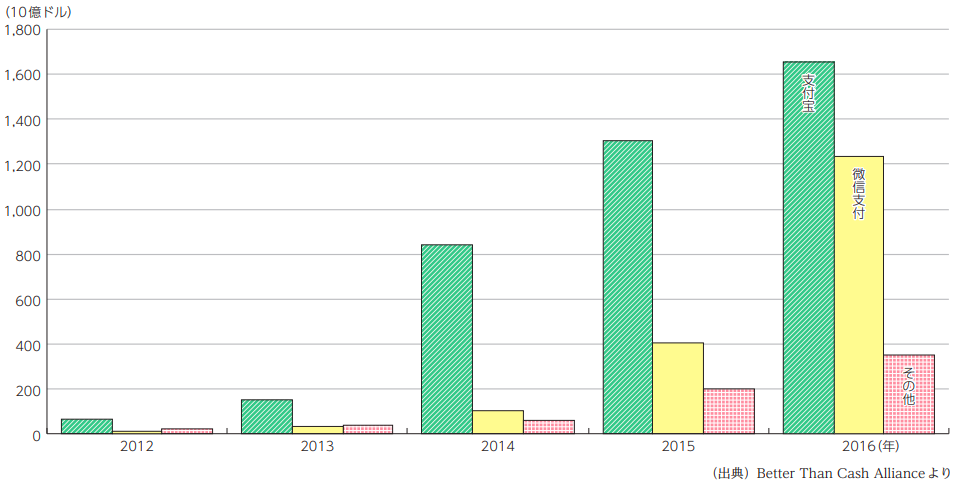
\includegraphics[width=13cm]{./imgs/1.png}
  \caption{中国におけるモバイル決済の市場規模比較}
\end{figure}

 中国のモバイル決済においては,支付宝(アリペイ)と微信支付(ウィーチャットペイ)が2大サービス提供者となっている.\\
 図1を見ると,支付宝では2012年の決済金額は700億ドルであったが,2016年度の決済金額は1兆7000億ドルであった.すなわち,4年間で決済金額はは24.3倍増加したと言える.また,ライバルサービスである微信支付では2012年の決済金額は116億ドルであり,4年後には1兆2000億ドル(2012年の100倍以上)まで成長した.\\
 なお,2017年12月現在,両者は全モバイル決済市場の90%以上シェアを占めている.\\

\newpage

 次に,日本と中国のATM設置台数を比較する.\\
\begin{figure}[H]
  \centering
  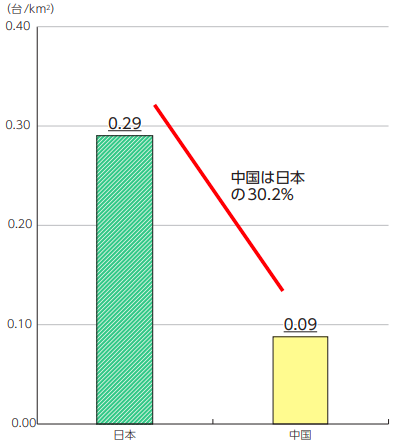
\includegraphics[width=5cm]{./imgs/2.png}
  \caption{中国におけるモバイル決済の市場規模比較}
\end{figure}
 図2\footnote{総務省 平成30年版情報通信白書 第2章 補論 中国の事例 図表3,\\http://www.soumu.go.jp/johotsusintokei/whitepaper/ja/h30/pdf/n2700000.pdf,2019-4-10閲覧}は,国土面積あたりのATM設置台数である.日本では0.29$\mbox{台/km}^2$であるのに対し、中国では0.09$\mbox{台/km}^2$と、3倍以上の開きがあることがわかる.\\

 また,中国では偽札が多く出回っており,銀行のATMから偽札が引き出されるケースもまれに発生している.\footnote{外務省 海外安全ホームページ: 安全対策基礎データ 中華人民共和国(中国),2019-4-12閲覧}\\

 以上の事実から,中国においてモバイル決済が急速に発展した理由について考察する.\\
 まず,考えられる理由として,サービス開始にかかるコストである.従来の銀行のネットワークシステムは整備に莫大な費用がかかる上に,多くの人手や時間がかかる.しかし,モバイル決済のシステムはインフラ整備をほとんど必要とせず,インターネットへの接続が可能な機器と,ネットワーク環境があれば導入することが容易である.経済的,時間的なコストが低いことがモバイル決済の普及に繋がった一番の要因であったと考える.\\
 加えて,ATMの設置状況は日本と比較すると劣っている.ATMの設置状況が悪ければ,現金を入手する際に不便である.しかし,モバイル決済を使用すれば,わざわざ現金を用意することなく,買い物をすることが可能となる.中国国内の現金入手性もまたモバイル決済の発展に寄与したと考えることができる.\\
 また,中国では偽札が多く出回っていることもモバイル決済の普及に影響を与えていると考えられる.偽札が多いということは,現金の信用が低いということである.現金よりも確実性のあると考えられ,普及を後押ししたと考えられる.

\end{document}
